\documentclass[prb,preprint]{revtex4-1} 

\usepackage{amsmath}  
\usepackage{amsfonts} 
\usepackage{graphicx} 
\usepackage{gensymb}

\begin{document}

\title{Measurement of Faraday Rotation and Calculation of the Verdet Constant for a SF-59 Glass Rod}

\author{Frances Yang}
\email{fyang@smith.edu} 

\author{Isabel Lipartito}
\email{iliparti@smith.edu}
\affiliation{Department of Physics, Smith College, Northampton, MA 01063}

\date{\today}

\begin{abstract}
{We observed the Faraday effect, a shift in the polarization of light as it passes through medium subject to a magnetic field. The Verdet constant relates the change in the magnetic field to a change in the polarization.  Polarized light from a 650 nm laser was sent through a SF-59 glass rod surrounded by a solenoid. The light then passed through an rotatable polarizer and was detected by a photodiode. A lock-in amplifier was used on the photodiode output to reduce noise from background light and DC drift from the photodiode. We calculated the Verdet constant for the rod by varying the magnetic fields and measuring the relative polarization shift and the voltage shift at a particular polarizer angle. From two separate calculations, we found a Verdet constant of $17.54 \pm 1.12 \mathrm{~rad/T} \cdot \textrm{m}$ and $19.88 \pm 0.11 \mathrm{~rad/T} \cdot \textrm{m}$. Other colleagues performing the experiment found the Verdet constant to be between 19 and 23$\mathrm{~rad/T} \cdot \textrm{m}$ from using the first method and between 19 and 21$\mathrm{~rad/T} \cdot \textrm{m} $from using the second method.  In our paper, we address a possible systematic error that lead to our Verdet Constant being too low from the first method.
}
\end{abstract}

\maketitle 
\section{Aims}
{a.  To demonstrate the Faraday effect of the rotation of the plane of polarization of light as it travels through magnetic fields of different magnitudes.

b.  To calculate the Verdet constant relating the change in polarization angle to the change in magnetic field.}
\begin{equation}
\Delta \phi =V_{c} \Delta B L{_{sample}}
\end{equation}

\section{Introduction} 

{The Faraday Effect is a magneto-optical phenomenon in which light of a single wavelength, traveling through certain materials subject to a magnetic field, experiences a shift in the plane of polarization. These materials, called birefringent, have different refractive indices for the right and left circular polarizations of light. As light travels through the material, the relative phase angle between the two polarizations changes, rotating the overall polarization plane.

As shown in Equation 1, the Verdet Constant ($V_{c}$) relates the change in magnetic field of a medium to the change in polarization angle of the traveling light.  $V_{c}$ is specific to any medium.  There are two ways in which we can calculate $V_{c}$.  By Malus's Law, $I(\theta)$=$I_{0}*\cos^{2}(\theta)$, where $I$ is the intensity of measured light through a polarization filter of angle $\theta$ with respect to the maximal polarization angle.  Similarly, for voltage output, $V(\theta)$=$V_{0}*\cos^{2}(\theta)$.  Once we add into this set-up a magnetic field through which the light can travel, we will observe the voltage output equation to have a phase shift, $\theta$:  $V(\theta)$=$V_{0}*\cos^{2}(\theta+\phi)$.

\subsection{Method 1}

{One way to find $V_{c}$ is to notice that $\frac{\partial \theta}{\partial B}=\frac{\partial V}{\partial B}/ \frac{\partial V}{\partial \theta}$.     $V=V_{0}*\cos(\theta)^{2}$.  Therefore,  $ \frac{\partial V}{\partial \theta} = V_{0}*\sin(2*\theta)$, or $V_{0}$, the amplitude of our voltage vs. angle plots, if $\theta$ is 45$\degree$.  $\frac{\partial V}{\partial B}$ can be found by plotting V(45$\degree$) against varying values of B. }

\begin{equation}
V_{c} =\frac{1}{L} * \frac{\partial V}{\partial B} /  \frac{\partial V}{\partial \theta} 
\end{equation}

\subsection{Method 2}

Another way to calculate $V_{c}$ is to measure the phase shift, $\phi$ for multiple magnetic fields:  collecting data for $V(\theta)$ for a full 0-360 degree range of $\theta$ and comparing data for different magnetic fields to a base data set of the same set up, where there is no magnetic field.  $\theta$ can be plotted against $B$- they should have a linear relationship- and by finding the slope of that linear fit, $\frac{\partial \theta}{\partial B}$ will be found and thus $V_{c}$ by Equation 1. We thus have another way to find the Verdet Constant.}

\begin{equation}
V_{c} =\frac{1}{L} * \frac{\partial \theta}{\partial B} 
\end{equation}



\section{Procedure}
{Polarized light came from a 650 nm laser, driven by a 400 kHZ square wave from a function generator. A 15.2 cm long solenoid with 1400 turns and a DC resistance of 1.6 $\Omega$ was the source of our magnetic field. The solenoid was connected to a Keithley 2230-30-1 DC Power Supply. Channel 1 and Channel 2 were connected in parallel to provide sufficient current. The calibration of the solenoid was found by measuring the magnetic field at the center of the solenoid for a current of 0 A to 2.25 A in steps of 0.25 A. The calibration constant was calculated to be $10.6 \textrm{~mT/A} \pm 0.05 \text{~mT}$. A 10.2 $\pm$ 0.5 cm SF-59 glass rod, was centered inside the solenoid. The light is passed through a polarizer and detected by a photodiode, connected to a 1 k$\Omega$ resistor. The photodiode outputs a voltage signal proportional to the detected light intensity.

A lock-in amplifier was used so undesirable noise such as light from the environment and drift from the photodiode, can be removed from the signal. The output of the photodiode was connected to a band pass filter with a center frequency of 400 kHz and a Q of 20. This extracted the first harmonic of the square wave, a 400 kHz sine wave. The output of of the filter was connected to a lock-in amplifier of gain 5. The reference signal for the lock-in amplifier was a 400 kHz sine wave with the same phase as the square wave driving the laser. It was generated by the same function generator for the square wave. The voltage output signal from the lock-in was measured by a Keithley 2100 Digital Multimeter.

Voltage readings from the multimeter were recorded onto the computer by LabView program (Keithley DC Incremental Write.vi). Each recorded voltage was an average of 16 measurements. Voltages were recorded for a 360\degree\ rotation of the polarizer at increments of 5\degree. We used this procedure to measure the voltage output for a magnetic field of -10.6 mT, 0 mT, 15.9 mT, and 21.2 mT. The negative field was generated by reversing the connection of the two leads of the power supply to the solenoid.
}




\section{Results}
{Data recorded by LabView was fed into a data analysis program called Igor.Pro.  A sinusoidal fit was determined for each separate dataset corresponding to a different current value.  We excluded two points in the curve fit for the B=0 dataset, which corresponded to values we accidentally recorded twice. 
We noticed something that, present in all data sets, the experimental measurements of voltage for angle settings of 305\degree--330\degree were systematically higher than the values predicted by the sinusoidal curve fit, resulting in our experimental curve to be shifted from the fit.  After the 330\degree mark, we noticed that our experimental data values began to agree once again with the sinusoidal fit.  In our Discussion section, we discuss possible causes for this systematic error.  In order to eliminate it as much as possible, we masked the values corresponding to angles of 305\degree--330\degree were masked from the curve fits as well for all datasets.
\begin{figure}
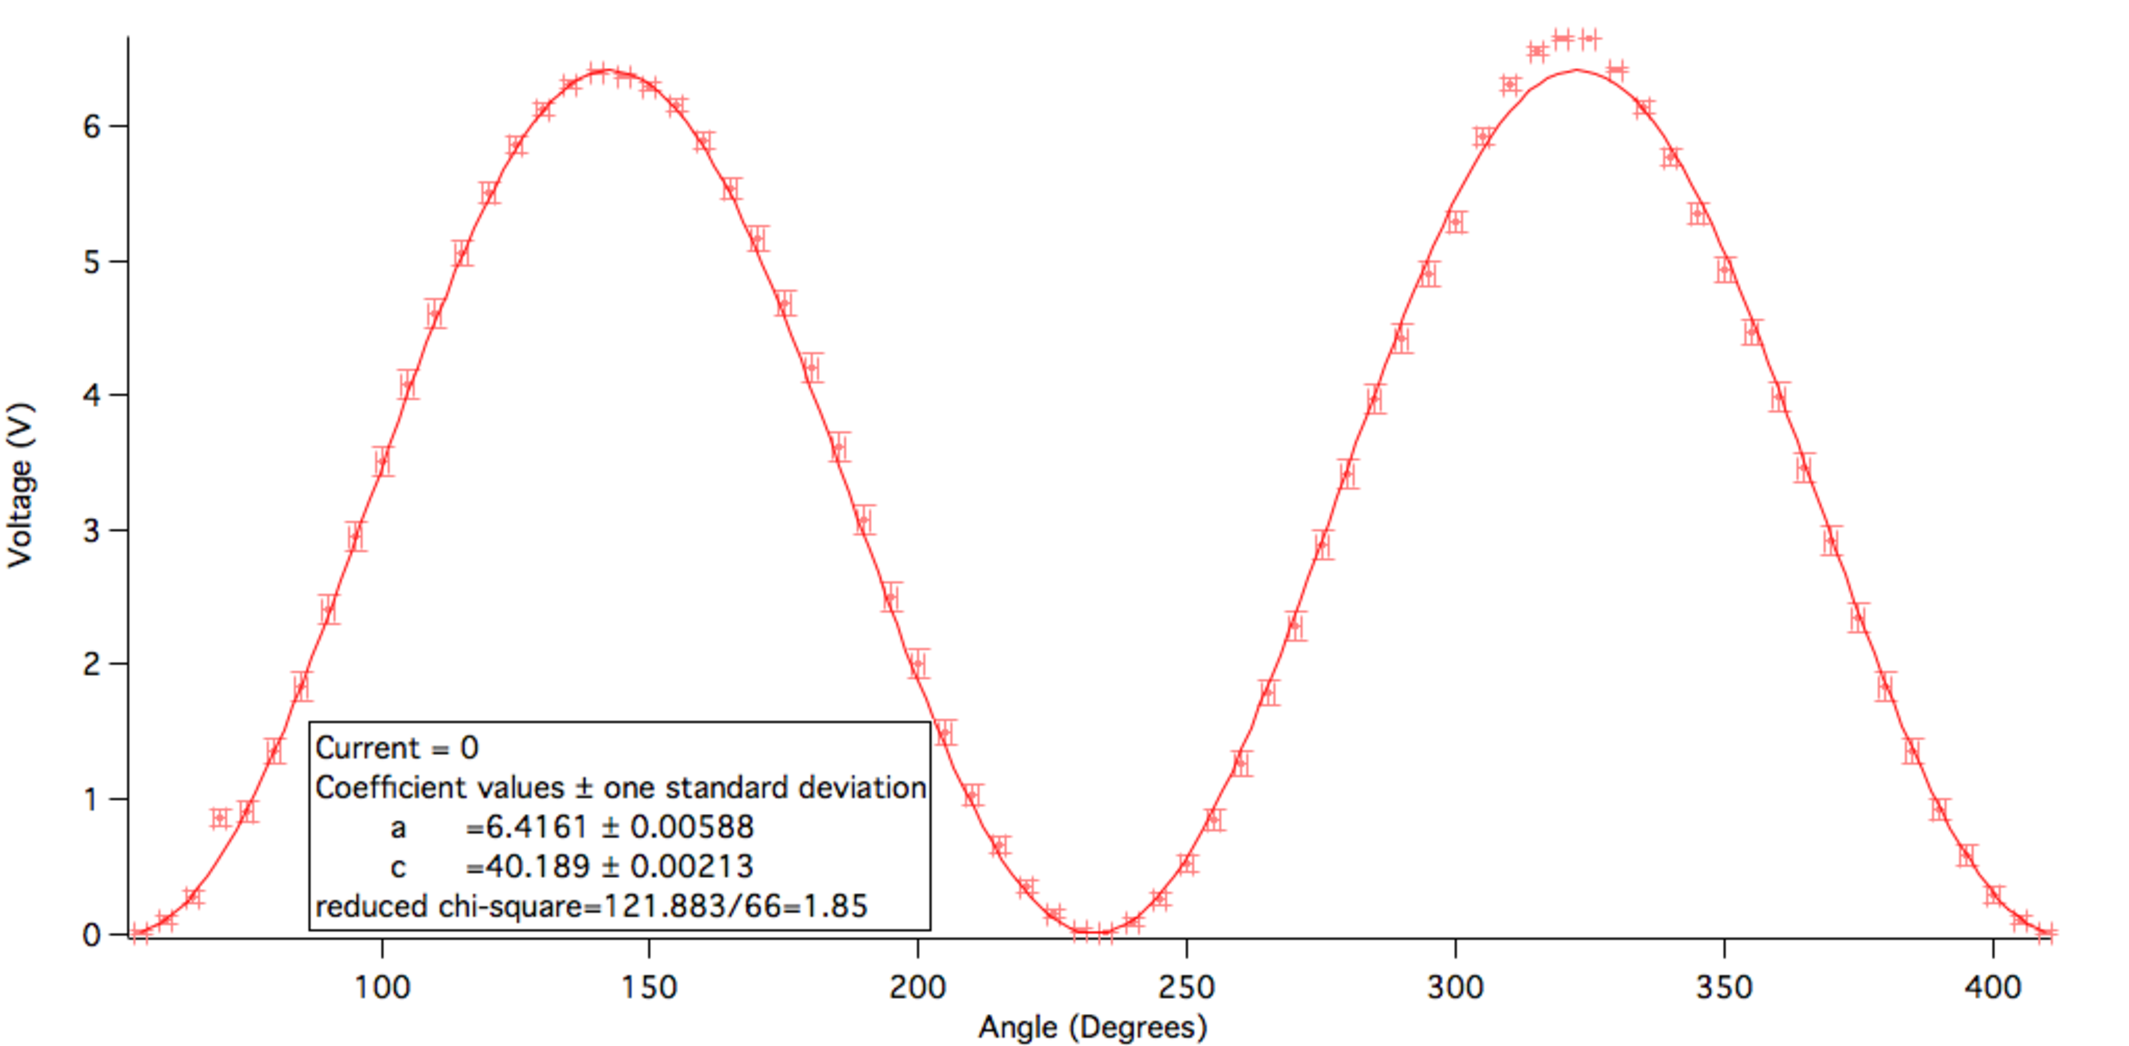
\includegraphics[width = 6.3in]{0A.pdf}
\caption{\label{nofield}Voltage measurements }

\end{figure}

\begin{figure}[b]
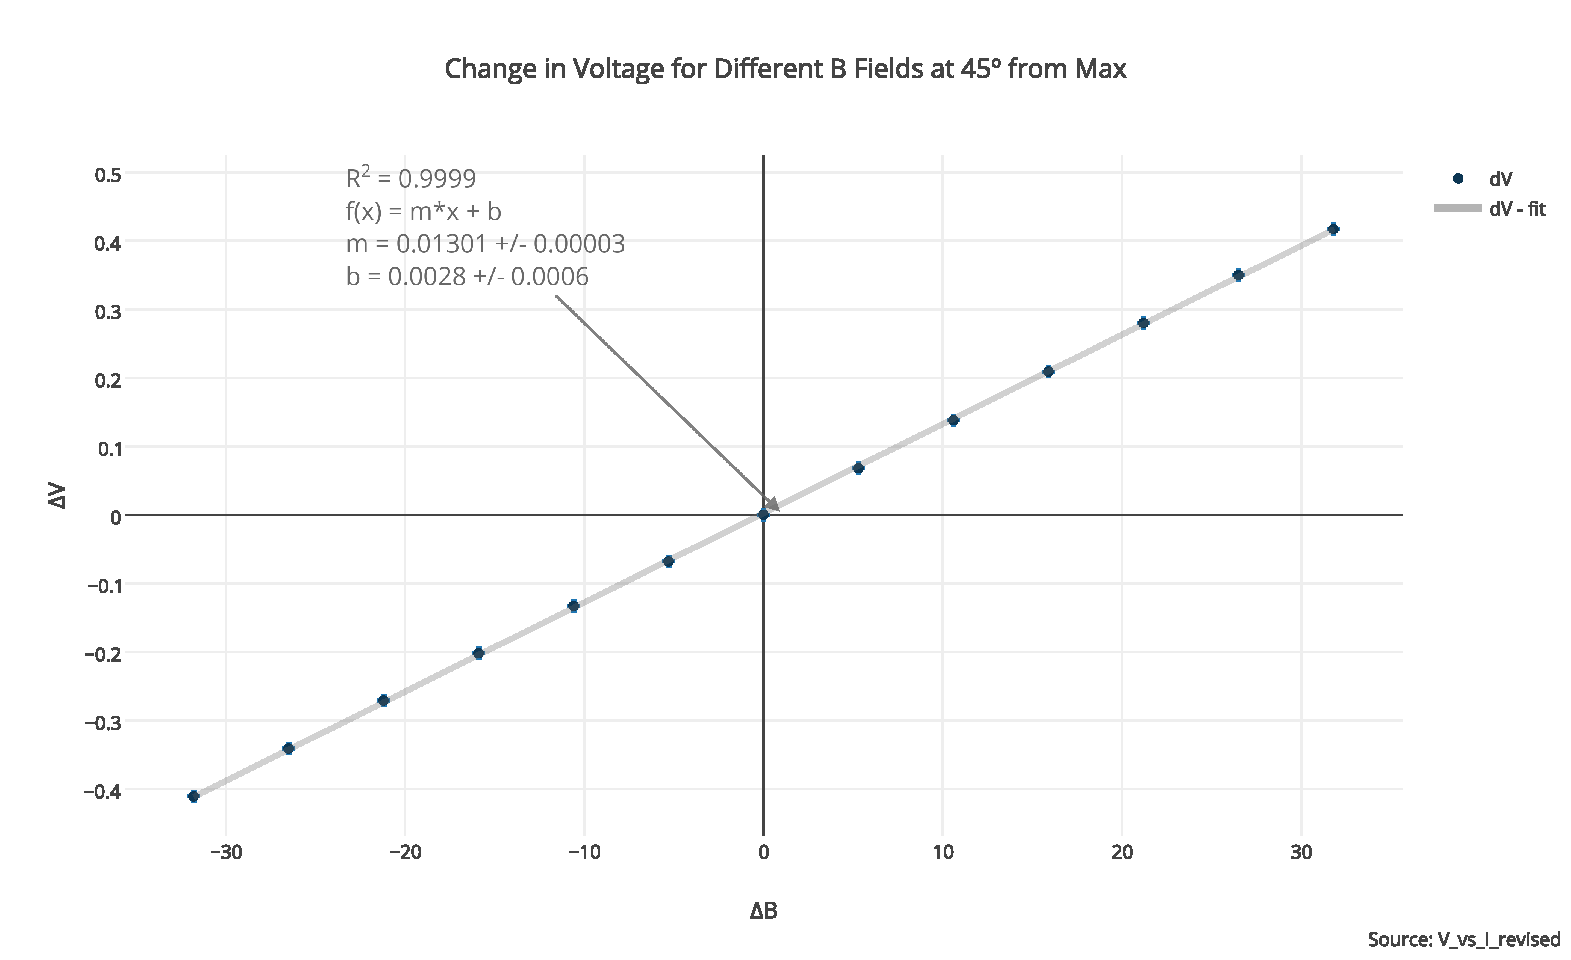
\includegraphics[width =6.3in]{change_in_voltage_for_different_b_fields_at_45_from_max.pdf}
\caption{\label{method2pic} The measured change in photodiode voltage for a change in the magnetic field at a polarizer angle 45\degree\  from the maximum voltage output. A linear fit was used to determine $\Delta V/\Delta B$.}
\end{figure}
}
\section{Analysis}
{We first calculated the Verdet Constant using the procedure detailed in Method 1.  We measured the value of V for multiple values of B generated by varying the current output I (-3.0 A to 3.0 A with increments of .5 A).  We plotted V vs B and found the slope of the curve and thus $\frac{\partial V}{\partial B}$ to be .013.  $\frac{\partial V}{\partial \theta}$, or $V_{0}$ at 45 $\degree$ was estimated to be (VALUE).  Error was taken to be 1 degree in setting the rotator to 45 $\degree$.  Applying Equation 2, we find the Verdet Constant to be $19.88 \pm 1.2 \mathrm{~rad/T} \cdot \textrm{m}$. (INSERT PLOT AT IMAGE).
{We then calculated the Verdet Constant using Method 2, which required we refer to the phase shifts from the four graphs of voltage vs angle set on the polarizer.  Using Igor.Pro, we generated a sinusoidal fit for the dataset of voltage vs. polarizer angle for all the B field settings.  Subtracting the fit for the zero B field setting from all the other fits, we were able to find the phase offset between the zero B field case and the three non-zero B field cases.  We generated a plot of voltage vs phase offset.  $\bf (Table)$.  The error in our curve-fitting program's calculation of the phase offset was used as the error in the offset.  The slope, and thus $\frac{\partial \theta}{\partial B}$ was measured to be .00179 $\pm$ .0000735 radians.  Applying Equation 3, we find that the Verdet Constant is $17.54 \pm 1.12 \mathrm{~rad/T} \cdot \textrm{m}$

\section{Discussion}

{We compared our values for the Verdet Constant with those found by colleagues performing the same experiment.  Using Method 1, our colleagues found the $V_{c}$ to be between 19 and 21$\mathrm{~rad/T} \cdot \textrm{m}$.  Our $V_{c}$ using Method 1, $19.88 \pm 1.2 \mathrm{~rad/T} \cdot \textrm{m}$ is thus in good agreement with the values of our fellow researchers as it falls within that range, within error.

{Our fellow colleagues found the value of the $V_{c}$ to be between 19 and 23 $\mathrm{~rad/T} \cdot \textrm{m}$.  Our value of $17.54 \pm 1.12 \mathrm{~rad/T} \cdot \textrm{m}$ is NOT within this range, including error, for one standard deviation.  We thus consider systematic errors present in our data which would have generated an inaccurate value using Method 2.  The most likely parameter which went into Equation 3 that could exhibit a systematic error is our calculation of $\partial \theta/\partial B$.  It is possible a systematic error was present in our measurement of the phase shift offset.  We remarked earlier that the 305\degree--330\degree regions of all four of our datasets were offset from the sinusoidal fit, due to what appears to be a systematic error in data collection.  In order to rectify this error, we had excluded those points from our curve fit. 



\section{Conclusion}


\section{References}


\end{document}
